\section{ Approach}
\label{sec:approach}
There are two steps in our approach, translation and revision.

\subsection{Translation}
Since both \pro and \con have the same triple form (node1, relation, node2), we do not differentiate their structures in this section.

%\KZ{Be careful of capitalization at the beginning of sentences.}
Multi-word expressions (MWEs) are semantically less ambiguous 
than mono-words \cite{finlayson2011detecting}, hence we treat MWEs as unambiguous terms.
We translate the triples with MWEs on both sides directly by 
packing two nodes together.
For example, given a triple, (``culture shock'', IsA, ``culture issue''), 
in order to give the translator a richer context, we first pack it into a 
contextual sentence with the comma separator (the comma is always kept in the translation result), such as ``culture shock, culture issue''.
Then, we put this contextual sentence into the translator.
Last, we unpack the translated result by the comma separator to assemble 
the corresponding Chinese triple.
Since the direct translation of triple containing at least one mono-word node 
cannot properly disambiguate word senses, as analyzed in Section \ref{sec:intro}, we design 
a revision method below.

\subsection{Revision}

The approach is shown in Figure \ref{fig:approach}. 
First, given one triple containing at least one mono-word node, such as (``date'', IsA, ``fruit''), 
we enumerate all the Chinese word senses of ``date'' and ``fruit'' respectively.
We feed each node into the translator
and obtain all the different translations.
For word ``fruit'', we can get all its Chinese word senses ``水果'', ``果实'', ``果'', ``果类'', etc. 
For word ``date'', we can get all its Chinese word senses ``日期'',``约会'',``枣''. 
It doesn't matter even if we retrieve semantically duplicated Chinese word senses,
because the translation with similar word senses will get close similarity, 
and it has no effect on the subsequent ranking results.
Then, calculate the similarities using the pre-trained word embedding between the Chinese word senses of these two nodes in the triple.
For the Chinese word sense of multi-word node, we segment them into words\footnote{Here, we use Jieba to segment Chinese text} and average their word embeddings
Last, rank the Chinese word sense node1-node2 pair according to the similarities,
and select the most similar Chinese word sense pair, such as (``枣/jujube'', ``水果/fruit''), as the translation result.
We use the Chinese Wikipedia dump on Aug 1, 2018, 
to train word embedding with Word2Vec tool\footnote{\url{https://code.google.com/archive/p/word2vec/}}.

\begin{figure}[ht]
	\centering
	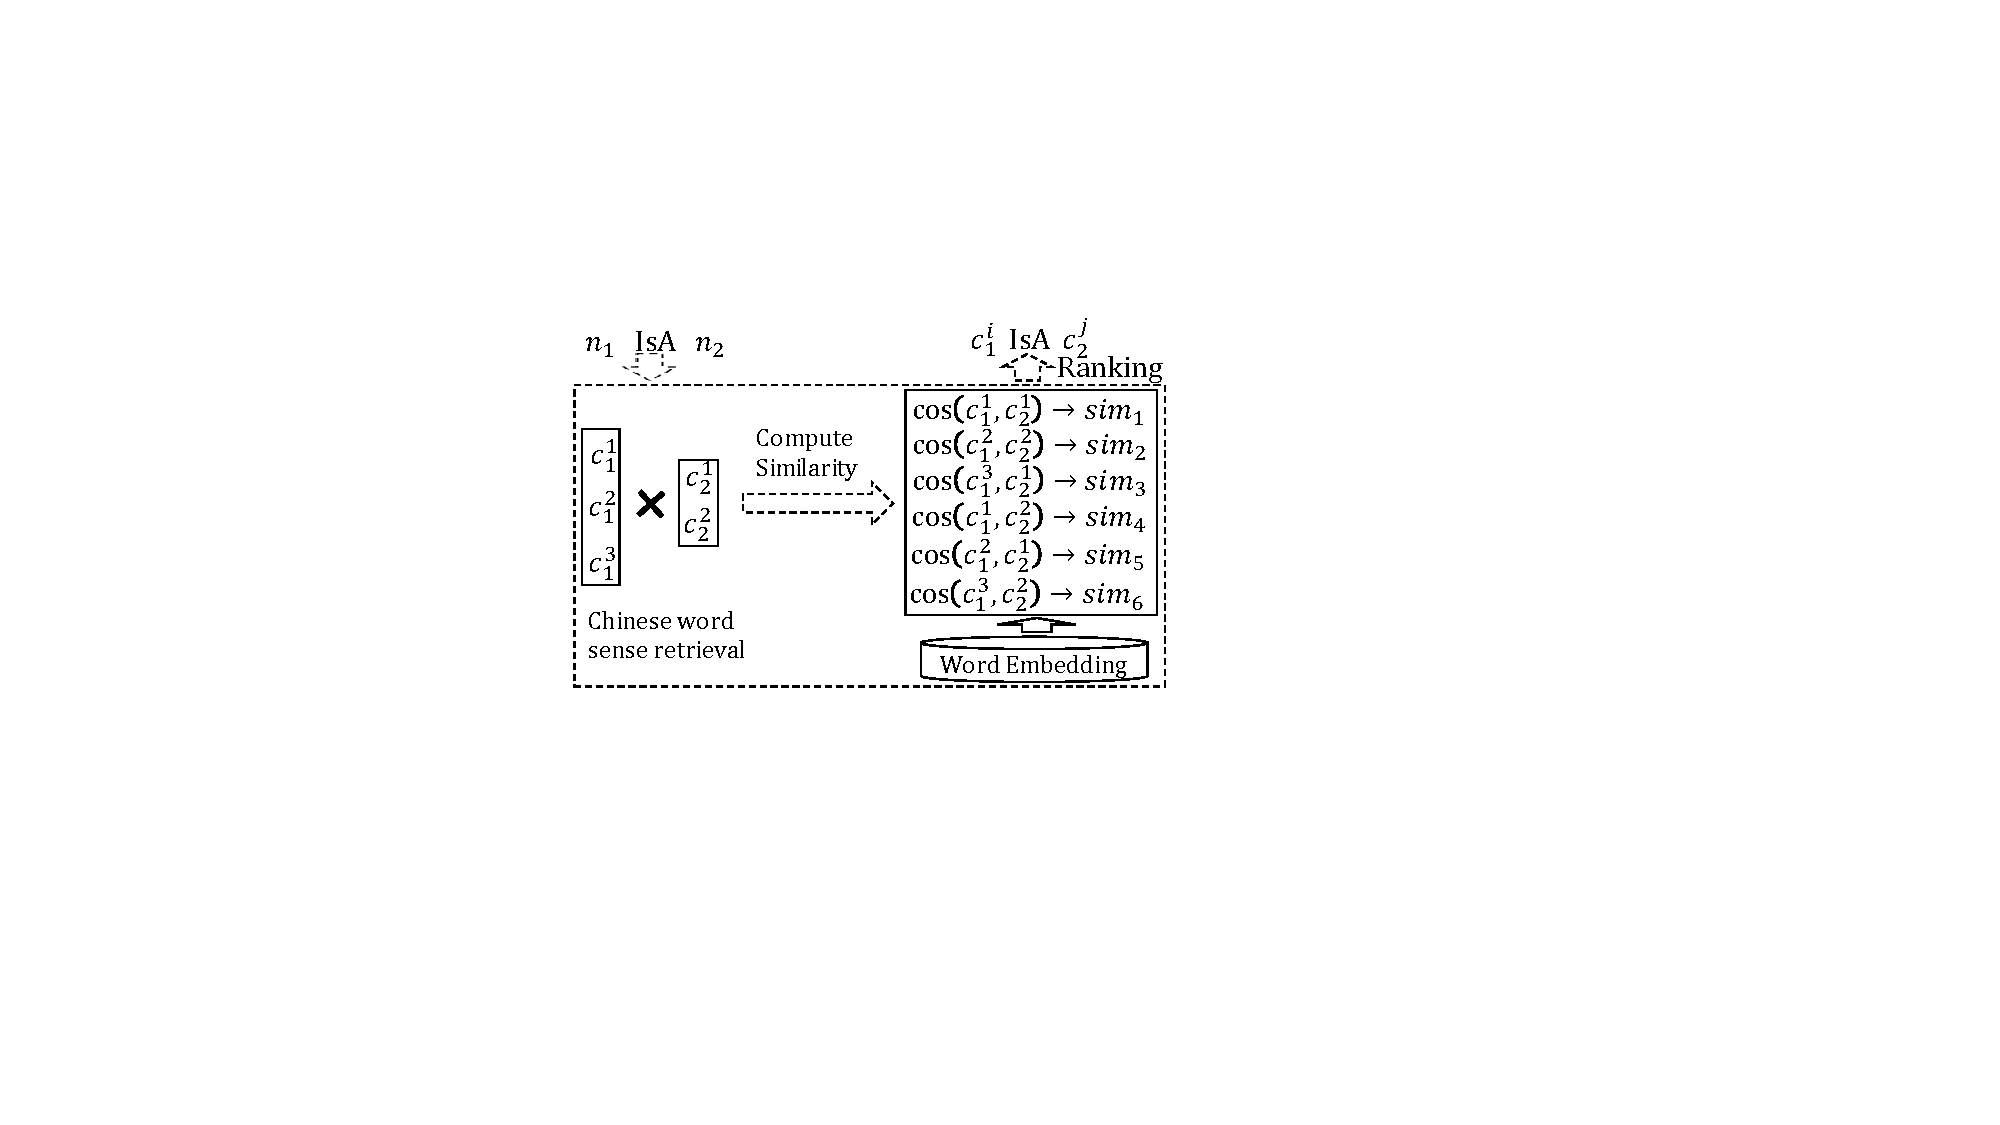
\includegraphics[width=\columnwidth]{figures/approach}
	\caption{Overall approach.}
	\label{fig:approach}
\end{figure}